\documentclass{beamer}

\usetheme{simple}

\usepackage{scalerel,xparse}
\usepackage{lmodern}
\usepackage[scale=2]{ccicons}
\usepackage{ulem}
\usepackage{tikz}
\usetikzlibrary{positioning,calc,automata}
\usepackage{algorithm}
\usepackage{algorithmic}
\usepackage{caption}
\usepackage{listings}
\usepackage{xcolor, enumitem}
\usepackage{hyperref}

% Watermark background (simple theme)
\setlength{\parindent}{0cm}
\setwatermark{
\includegraphics[height=8cm]{img/chungus.png}}

\NewDocumentCommand\emojisushi{}{
    
\includegraphics{img/1f363.png}
}
\NewDocumentCommand\emojicarrot{}{
    
\includegraphics[width=0.3cm]{img/1f955.png}
}   
\NewDocumentCommand\emojijuice{}{
    
\includegraphics[width=0.3cm]{img/1f9c3.png}
}   
\NewDocumentCommand\emojibaguette{}{
    
\includegraphics[width=0.3cm]{img/1f956.png}
}   
\NewDocumentCommand\emojicroissaint{}{
    
\includegraphics[width=0.3cm]{img/1f950.png}
}   
\NewDocumentCommand\emojionigiri{}{
    
\includegraphics[width=0.3cm]{img/1f359.png}
}   


\title{CSC363 Tutorial 11}
\subtitle{almost done!}
\date{\today}
\author{Paul ``sushi{\textunderscore}enjoyer'' Zhang}
\institute{University of Chungi}

\begin{document}

\maketitle

\begin{frame}{Learning objectives this tutorial}
By the end of this tutorial, you should...
\begin{itemize}
\item Have one more NP-complete problem added to your ``NP-complete problems'' toolkit.
\item Add a problem to your ``NP-hard problems'' toolkit, even though it's kinda useless since the problem isn't even computable.
\item Probably work on assignment 5? Oh wait, you probably have other courses with higher priority... :(
\item Be scared for the final exam! D:
\item Feel like sushi\_enjoyer is just being sarcastically enthusiastic about CSC363 material when he himself hates it.
\end{itemize}

Big Chungus certified readings: chapter 8 probably, but it isn't really necessary tbh.
\end{frame}

\begin{frame}{do you like proving NP-completeness? D:}
well too bad! you'll have to do it for the upcoming problem set.

\begin{figure}[h]
\centering

\includegraphics[width=8cm]{img/oooooooooooooooooooooooooooooooooooooooooooooooooohhhhhh.png}
\end{figure}
\end{frame}

\begin{frame}{Set cover}
We will now describe the \textbf{set cover problem} and prove it is NP-complete, because why not.

\vspace{2mm}

Suppose we are given a set of elements $U$ (called the \textit{universe}), and a collection $\mathcal S = \{S_1, \ldots, S_n\}$ of subsets of $U$ such that (brace yourself, $\bigcup$)
$$\bigcup_{i = 1}^n S_i = U.$$
A \textbf{set cover} of $U$ is a subcollection $\mathcal S' = \{S_{i_1}, S_{i_2}, \ldots, S_{i_k}\} \subseteq \mathcal S$ such that $$\bigcup_{m = 1}^k S_{i_k} = U.$$

For example, if $U = \{1, 2, 3, 4, 5\}$, and our collection of sets is $\mathcal S = \{\{1, 2, 3\}, \{2, 4\}, \{3, 4\}, \{4, 5\}\}$, then $\{\{1, 2, 3\}, \{4, 5\}\}$ is a set cover.
\end{frame}

\begin{frame}{Set cover}
\textbf{Task:} Let $U = \{\emojisushi, \emojijuice, \emojicarrot, \emojicroissaint, \emojibaguette, \emojionigiri\}$, and $$\mathcal S = \{\{\emojisushi, \emojibaguette\}, \{\emojijuice, \emojibaguette, \emojionigiri\}, \{\emojijuice, \emojicarrot, \emojibaguette\}, \{\emojicroissaint, \emojionigiri\}, \{\emojicroissaint\}, \{\emojisushi, \emojicarrot, \emojicroissaint\}\}.$$
Find the smallest set cover of $U$.

\textbf{Answer:} The smallest set cover is $\{\{\emojijuice, \emojibaguette, \emojionigiri\}, \{\emojisushi, \emojicarrot, \emojicroissaint\}\}$, which is of size 2.
\end{frame}

\begin{frame}{Set cover is NP-complete!}
Now given a universal set $U$, a collection $\mathcal S = \{S_1, \ldots, S_n\}$ of subsets of $U$, and a natural number $k$, the \textbf{set cover problem} asks you whether it is possible to find a set cover for $U$ of size $k$. In language form, it would be
\begin{align*}
\text{Set-Cover} = &\{(U, \mathcal S, k): \text{$U$ is a set, $\mathcal S$ is a collection of subsets of $U$,}\\
& \quad \text{and there is a set cover of $U$ of size $k$}\}.
\end{align*}

Turns out this problem is NP-complete! Let's prove it's NP first.

\textbf{Task:} Prove that Set-Cover is NP.
\end{frame}

\begin{frame}{Set cover is NP-complete!}
\textbf{Task:} Prove that Set-Cover is NP.

\vspace{2mm}

\textbf{Answer:} We can build a poly-time verifier $V$ that checks whether a given subcollection $\mathcal S'$ of $\mathcal S$ is a set cover for $U$.
\begin{align*}
V(U, \mathcal S, k, \mathcal S'): \quad &\text{Check if $\mathcal S' \subseteq \mathcal S$}\\
&\text{Check if $\bigcup_{S_i \in \mathcal S'} S_i = U$}\\
&\text{Check if $|\mathcal S'| = k$}\\
&\text{Accept iff all of the above are true}
\end{align*}
Now we prove it is NP-complete. Remember how we can prove something is NP-complete by showing that some known NP-complete problem reduces to it?
\end{frame}

\begin{frame}{Set cover is NP-complete!}
Now we prove it is NP-complete. Remember how we can prove something is NP-complete by showing that some known NP-complete problem reduces to it?

\textbf{Task:} Show that $\text{Set-Cover} \in \text{NP}$ by proving $\text{Vertex-Cover} \leq_p \text{Set-Cover}$.\footnote{Recall: this involves converting an instance of the vertex cover problem into an instance of set cover problem in poly-time.}
\end{frame}

\begin{frame}{Set cover is NP-complete!}
\textbf{Answer:} Suppose we are given an instance $(G, k)$ of the vertex cover problem. We may transform it into a set cover problem $(U_G, \mathcal S_G, k_G)$ with the property that $$(G, k) \in \text{Vertex-Cover} \Leftrightarrow (U_G, \mathcal S_G, k_G) \in \text{Set-Cover}.$$
Let $v_1, \ldots, v_n$ be the vertices of $G$, and $e_1, \ldots, e_m$ the edges of $G$. Define $U_G, \mathcal S_G, k_G$ as follows: 
\begin{itemize}
\item $U_G$ will consist of all the edges $\{e_1, \ldots, e_m\}$.
\item For each vertex $v_i$, let $S_i$ be the set of edges that $v_i$ touches. Then let $\mathcal S_G = \{S_1, \ldots, S_n\}$.
\item $k_G = k$.
\end{itemize}
This transformation takes poly-time with respecc to the size of $(G, k)$.
We claim $(G, k) \in \text{Vertex-Cover} \Leftrightarrow (U_G, \mathcal S_G, k_G) \in \text{Set-Cover}$.
\end{frame}

\begin{frame}{Set cover is NP-complete!}
    We'll ``prove'' $(G, k) \in \text{Vertex-Cover} \Leftrightarrow (U_G, \mathcal S_G, k_G) \in \text{Set-Cover}$ via example.\footnote{Please, please, please,  \textbf{do not do this in any proof course}. It's just easier for illustrate with an example.} Suppose $k = 2$ and $G$ is the following graph:
\begin{center}
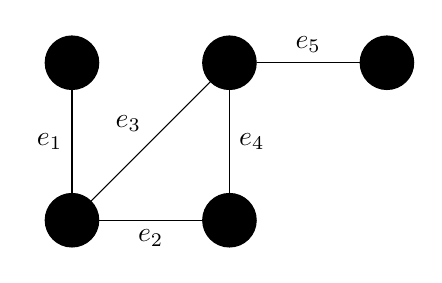
\begin{tikzpicture}[vertex/.style={circle,draw,fill=black,minimum size=3mm,inner sep=3pt]}]
\node[vertex] (v1) at (0, 0) {$v_1$}; 
\node[vertex] (v2) at (0, 2) {$v_2$}; 
\node[vertex] (v3) at (2, 0) {$v_3$}; 
\node[vertex] (v4) at (2, 2) {$v_4$};
\node[vertex] (v5) at (4, 2) {$v_5$};
\draw (v1) -- (v2) node[midway, left] {$e_1$};
\draw (v1) -- (v3) node[midway, below] {$e_2$};
\draw (v1) -- (v4) node[midway, above left] {$e_3$};
\draw (v3) -- (v4) node[midway, right] {$e_4$};
\draw (v4) -- (v5) node[midway, above] {$e_5$};
\end{tikzpicture}
\end{center}
\begin{itemize}
\item $U_G$ will consist of all the edges $\{e_1, \ldots, e_m\}$.
\item For each vertex $v_i$, let $S_i$ be the set of edges that $v_i$ touches. Then let $\mathcal S_G = \{S_1, \ldots, S_n\}$.
\item $k_G = k$.
\end{itemize}
\textbf{Task:} Find $U_G$, $\mathcal S_G$, and $k_G$ for this instance of the vertex cover problem.
\end{frame}

\begin{frame}{Set cover is NP-complete!}
\begin{center}
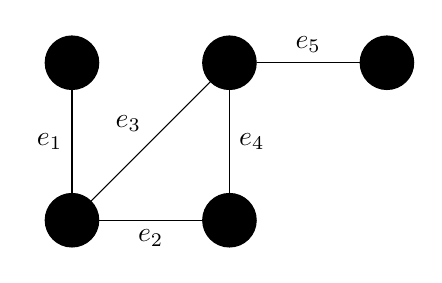
\begin{tikzpicture}[vertex/.style={circle,draw,fill=black,minimum size=3mm,inner sep=3pt]}]
\node[vertex] (v1) at (0, 0) {$v_1$}; 
\node[vertex] (v2) at (0, 2) {$v_2$}; 
\node[vertex] (v3) at (2, 0) {$v_3$}; 
\node[vertex] (v4) at (2, 2) {$v_4$};
\node[vertex] (v5) at (4, 2) {$v_5$};
\draw (v1) -- (v2) node[midway, left] {$e_1$};
\draw (v1) -- (v3) node[midway, below] {$e_2$};
\draw (v1) -- (v4) node[midway, above left] {$e_3$};
\draw (v3) -- (v4) node[midway, right] {$e_4$};
\draw (v4) -- (v5) node[midway, above] {$e_5$};
\end{tikzpicture}
\end{center}
\begin{itemize}
\item $U_G = \{e_1, e_2, e_3, e_4, e_5\}$.
\item We have $S_1 = \{e_1, e_2, e_3\}$, $S_2 = \{e_1\}$, $S_3 = \{e_2, e_4\}$, $S_4 = \{e_3, e_4, e_5\}$, $S_5 = \{e_5\}$. So $$\mathcal S_G = \{S_1, \ldots, S_5\} = \{\{e_1, e_2, e_3\}, \{e_1\}, \{e_2, e_4\}, \{e_3, e_4, e_5\}, \{e_5\}\}.$$
\item $k_G = 2$ since $k = 2$.
\end{itemize}

\textbf{Task:} Find a vertex cover for $G$. What would the corresponding set cover be?
\end{frame}

\begin{frame}{Set cover is NP-complete!}
\begin{center}
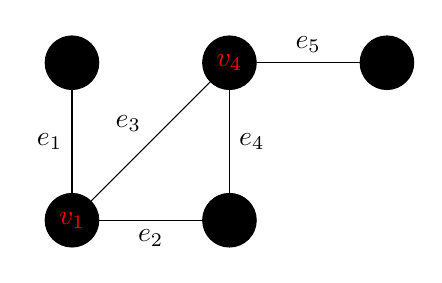
\begin{tikzpicture}[vertex/.style={circle,draw,fill=black,minimum size=3mm,inner sep=3pt]}]
\node[vertex] (v1) at (0, 0) {\color{red} $v_1$}; 
\node[vertex] (v2) at (0, 2) {$v_2$}; 
\node[vertex] (v3) at (2, 0) {$v_3$}; 
\node[vertex] (v4) at (2, 2) {\color{red} $v_4$};
\node[vertex] (v5) at (4, 2) {$v_5$};
\draw (v1) -- (v2) node[midway, left] {$e_1$};
\draw (v1) -- (v3) node[midway, below] {$e_2$};
\draw (v1) -- (v4) node[midway, above left] {$e_3$};
\draw (v3) -- (v4) node[midway, right] {$e_4$};
\draw (v4) -- (v5) node[midway, above] {$e_5$};
\end{tikzpicture}
\end{center}
\begin{itemize}
\item $U_G = \{e_1, e_2, e_3, e_4, e_5\}$.
\item We have $S_1 = \{e_1, e_2, e_3\}$, $S_2 = \{e_1\}$, $S_3 = \{e_2, e_4\}$, $S_4 = \{e_3, e_4, e_5\}$, $S_5 = \{e_5\}$. So $$\mathcal S_G = \{S_1, \ldots, S_5\} = \{\{e_1, e_2, e_3\}, \{e_1\}, \{e_2, e_4\}, \{e_3, e_4, e_5\}, \{e_5\}\}.$$
\item $k_G = 2$ since $k = 2$.
\end{itemize}
$v_1, v_4$ form a vertex cover of $G$. $\mathcal S' = \{S_1, S_4\}$ forms a set cover of $U$. 
\end{frame}

\begin{frame}{Break time!}
No sushi juice this time. But you get to ask me one question, about pretty much anything (as long as it's appropriate i guess lol).

\begin{figure}[h]
\centering

\includegraphics[width=5cm]{img/uwu.png}
\end{figure}
\end{frame}

\begin{frame}{no more brake time with uwu}
Alright so we now have one more problem that we know is NP-complete. I'm so excited! Anyone? ;-;

\vspace{2mm}

Let's add an NP-hard problem to the back of our memory! This one is actually a bit tricky to prove though...

\vspace{2mm}

\textbf{Task:} What does HP stand for?
\end{frame}

\begin{frame}{no more brake time with uwu}
\textbf{Task:} What does HP stand for?

\textbf{Answer:} \textbf{H}elo \textbf{P}hish.
\begin{figure}[h]
\centering

\includegraphics[width=7cm]{img/helo_fish.jpg}
\end{figure}
$$\text{HP} = \{(M, w): \text{$M$ is a Turing machine that halts on input $w$}\}.$$
We will prove HP is NP-Hard by showing $\text{3SAT} \leq_p \text{HP}$.\footnote{In fact, any computable language $A$ satisfies $A \leq_p \text{HP}$! You can just adapt the proof I'm about to show.}
\end{frame}

\begin{frame}{HP is NP-Hard}
$$\text{HP} = \{(M, w): \text{$M$ is a Turing machine that halts on input $w$}\}.$$
We will construct the following reduction of 3SAT to HP. Suppose $\varphi$ is a given instance of 3SAT. Construct the following Turing machine $M$:

\begin{align*}
M(\varphi): \quad &\text{Check whether $\varphi \in \text{3SAT}$ via brute force.}\\
&\text{If $\varphi \in \text{3SAT}$:}\\
&\quad \text{Accept}\\
&\text{Else:}\\
&\quad \text{Loop}
\end{align*}
Notice that \textit{it takes constant time to construct $M$}, since the \textit{code} of $M$ doesn't depend on $\varphi$ at all. It's like writing a program that writes a fixed Python script into a text file. Also, \textit{we don't run $M$; we only construct it, and bypass the exponential time computation needed to check whether $\varphi \in \text{3SAT}$ via brute force.} Again, it's like writing some really slow code to a text file but not running it.

\end{frame}

\begin{frame}{HP is NP-Hard}
$$\text{HP} = \{(M, w): \text{$M$ is a Turing machine that halts on input $w$}\}.$$
We will construct the following reduction of 3SAT to HP. Suppose $\varphi$ is a given instance of 3SAT. Construct the following Turing machine $M$:

\begin{align*}
M(\varphi): \quad &\text{Check whether $\varphi \in \text{3SAT}$ via brute force.}\\
&\text{If $\varphi \in \text{3SAT}$:}\\
&\quad \text{Accept}\\
&\text{Else:}\\
&\quad \text{Loop}
\end{align*}

\textbf{Task:} Show $\varphi \in \text{3SAT} \Leftrightarrow (M, \varphi) \in \text{HP}$, where $M$ is as above. Then convince yourself that we can replace 3SAT with any computable language, and the same proof would work.

\end{frame}




\begin{frame}{buy}
\texttt{helo\_fish.jpg} is sad to see you go ;-; 

only one more week left! D:

\begin{figure}[h]
\centering

\includegraphics[width=7cm]{img/helo_fish_sad.jpg}
\end{figure}
\end{frame}




\end{document}